\documentclass[14pt,a4paper]{article}
\usepackage[latin1]{inputenc}
\usepackage[T1]{fontenc}
\usepackage[english]{babel}
\usepackage{amsmath}
\usepackage{amsfonts}
\usepackage{amssymb}
\usepackage{makeidx}
\usepackage{amsthm}
\usepackage{geometry}
\usepackage[linesnumbered,ruled]{algorithm2e}
\usepackage{tikz}
\usetikzlibrary{automata, positioning}
\usepackage{float}
\usepackage[round]{natbib}
\usepackage[hidelinks]{hyperref}
\usepackage{caption}
\usepackage{graphicx}
\usepackage{subcaption}
\usepackage{listings}
\usepackage{color}
\usepackage{ dsfont }
\usepackage[justification=centering]{caption}
\usepackage{eqnarray}

\makeatletter
\@addtoreset{section}{part}
\makeatother  


\let\oldpart\part
\renewcommand\part{\newpage\oldpart}

\def\code#1{\texttt{#1}}
\newtheorem{theorem}{Theorem}[section]
\def\iff{\Leftrightarrow}
\theoremstyle{definition}
\newtheorem{madef}{Definition}[section]
\newtheorem{prop}{Proposition}[section]
\newtheorem*{remark}{Remark}

 
\definecolor{codegreen}{rgb}{0,0.6,0}
\definecolor{codegray}{rgb}{0.5,0.5,0.5}
\definecolor{codepurple}{rgb}{0.58,0,0.82}
\definecolor{backcolour}{rgb}{0.95,0.95,0.92}

\lstdefinestyle{mystyle}{
    backgroundcolor=\color{backcolour},   
    commentstyle=\color{codegreen},
    keywordstyle=\color{magenta},
    numberstyle=\tiny\color{codegray},
    stringstyle=\color{codepurple},
    basicstyle=\footnotesize,
    breakatwhitespace=false,         
    breaklines=true,                 
    captionpos=b,                    
    keepspaces=true,                 
    numbers=left,                    
    numbersep=5pt,                  
    showspaces=false,                
    showstringspaces=false,
    showtabs=false,                  
    tabsize=2
}
 
\lstset{style=mystyle}



%to hide the todos or to show them
%\usepackage[colorinlistoftodos,prependcaption,obeyDraft]{todonotes}
\usepackage[colorinlistoftodos,prependcaption]{todonotes}


\usepackage{xargs}                      % Use more than one optional parameter in a new commands
\newcommandx{\unsure}[2][1=]{\todo[linecolor=red,backgroundcolor=red!65,bordercolor=red,#1]{#2}}
\newcommandx{\change}[2][1=]{\todo[linecolor=blue,backgroundcolor=blue!25,bordercolor=blue,#1]{#2}}
\newcommandx{\info}[2][1=]{\todo[linecolor=OliveGreen,backgroundcolor=OliveGreen!25,bordercolor=OliveGreen,#1]{#2}}
\newcommandx{\improvement}[2][1=]{\todo[linecolor=Plum,backgroundcolor=Plum!25,bordercolor=Plum,#1]{#2}}
\newcommandx{\idea}[2][1=]{\todo[linecolor=green,backgroundcolor=green!25,bordercolor=green,#1]{#2}}



\numberwithin{equation}{subsection}

%\oddsidemargin  0in
%\evensidemargin  0in
%\textwidth   6.3in
%\textheight  9.5in
%\topmargin  -0.7in


\usepackage{fancyhdr}
\pagestyle{fancy}
%\lfoot{Charles DUFOUR}
%\rfoot{\today}
%\fancyhead[R]{}
\fancyhead[L]{}

\author{Charles Dufour}
\title{Bachelor Project: \\
Reinforcement learning and robot navigation}
\begin{document}

\begin{titlepage}
\newcommand{\HRule}{\rule{\linewidth}{0.5mm}} % Defines a new command for the horizontal lines, change thickness here

\center % Center everything on the page
 
%----------------------------------------------------------------------------------------
%   HEADING SECTIONS
%----------------------------------------------------------------------------------------

\vspace{3cm}
\textsc{\LARGE \'Ecole polytechnique f\'ed\'erale de Lausanne}\\[0.5cm] % Name of your university/college
\textsc{\large Disopt}\\[1.5cm] % Name of your university/college
\textsc{\LARGE Master semester project}\\[0.5cm] % Major heading such as course name
\textsc{\large Autumn Semester 2019 }\\[0.5cm] % Minor heading such as course title

%----------------------------------------------------------------------------------------
%   TITLE SECTION
%----------------------------------------------------------------------------------------

\HRule \\[0.4cm]
{ \huge \bfseries A combinatorial approach to the trains routing problem}\\[0.4cm] % Title of your document
\HRule \\[1.5cm]
 
%----------------------------------------------------------------------------------------
%   AUTHOR SECTION
%----------------------------------------------------------------------------------------

\begin{minipage}{0.4\textwidth}
\begin{flushleft} \large
\emph{Student:}\\
Charles Dufour
\end{flushleft}
\end{minipage}
~
\begin{minipage}{0.4\textwidth}
\begin{flushright} \large
\emph{Supervisors:} \\
Prof. Friedrich Eisenbrand \\% Supervisor's Name
Jonas Racine
\end{flushright}
\end{minipage}\\[5cm]

%----------------------------------------------------------------------------------------
%   LOGO SECTION
%----------------------------------------------------------------------------------------

 
\includegraphics[width=0.5\linewidth]{img/logo.eps}\\[1cm] % Include a department/university logo - this will require the graphicx package
 
%----------------------------------------------------------------------------------------

\vfill % Fill the rest of the page with whitespace


\end{titlepage}




\newpage





\tableofcontents
\pagenumbering{gobble}
\newpage






\pagenumbering{arabic}
\section*{Introduction}
\addcontentsline{toc}{section}{Introduction}
Presentation of the challenge that serves as experimental ground.

%\begin{figure}[H]
%\centering
%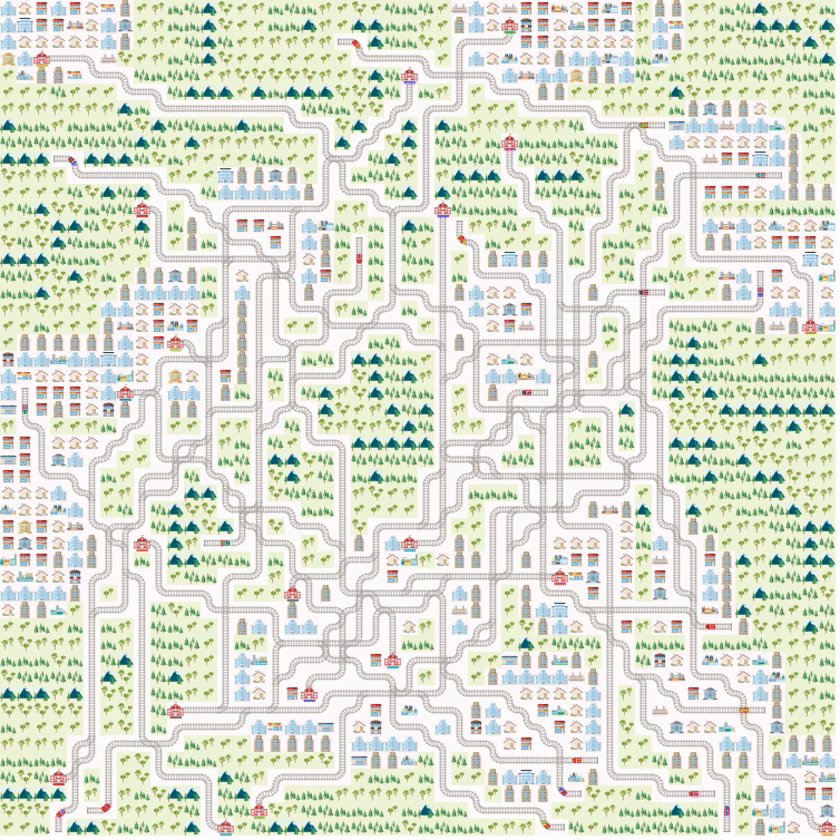
\includegraphics[scale=0.4]{img/flatland.png}
%\caption{Example of the railway network environment from the Flatland challenge}
%\end{figure}


\newpage
\section{Literature review}
\subsection{Double vertex graph}
\subsection{MAPF}


\newpage
\section{Modelization of the environment}
\subsection{Transition network}

The transition network is an oriented graph $G = (V,A)$ that represents the original 2D grid world.

\subsection{Time expanded network}
\label{ten}
We give a definition inspired from \cite[p.~19]{Skutella2008AnIT}:
\begin{madef}[Time-expanded network]
	 Let $G = (V, E)$ be a network with capacities $u$ and costs $c$ on the arcs. For a given time horizon $T\in \mathds{Z}_{>0}$ ,	the corresponding \emph{time-expanded network} $G^T = (V^T, E^T)$ with capacities and costs on the arcs
	is defined as follows. For each node $v\in V$ we create $T$ copies $v_0 , v_1 , \ldots, v_{T-1} $, that is,
	$$V^T := \{v_\theta | v \in V, \theta = 0, 1, \ldots, T-1\}.$$
	For each arc $e = (v, w) \in E$, there are $T-1$  copies $e_0,e_1,\ldots,e_{T-2}$ where arc $e_\theta$ connects
	node $v_\theta$ to node $w_{\theta+1}$ . Arc $e_\theta$ has capacity $u_{e_{\theta}}:= u_{e_\theta}$ and cost $c_{e_{\theta}}:= c_{e_\theta}$. Moreover, $E^T$ contains
	\emph{waiting} arcs $(v_\theta , v _{\theta+1})$ for $v \in V$ and $\theta = 0,\ldots, T-2$. The capacity of waiting arcs is $1$
	and they have cost $1$. Summarizing, the set of arcs $E^T$ is given by
	\begin{align*}
	 E^T := &\{e_\theta = (v_\theta,w_{\theta+1})| e = (u,v) \in E, \theta=0,1,\ldots,T-2 \} \\
	 &\cup \{(v_\theta,v_{\theta+1})|v\in V, \theta=0,1,\ldots,T-2 \}
	 \end{align*}
\end{madef}

An example of a time-expanded network is given in Figure \ref{fig:timeExpandedNetwork}. Notice that the size of the	time-expanded network $G^T$ is linear in $T$ and therefore only pseudo-polynomial in the input
size.


We then proceed to define a time step, which represent what would be added to a time expanded graph, were we to expand the horizon by one.

\begin{madef}[Time step in time expanded network]	
	A \emph{time step} at time $\theta$ is the set of all edges $(v_\theta,w)$ for all $v \in V$, $w \in V^T$ such that $(v_\theta,w) \in E^T$. 
	It represents the set of all edges starting at time $\theta$.
\end{madef}

\todo[inline]{explain a bit more}
\todo[inline]{add an example as a Figure}


\begin{remark}
	There are no cycles in the time expanded network since $\nexists (v_\theta,w_{\tilde{\theta}}) \in E^T$ with $\tilde{\theta} < \theta$.
\end{remark}
	
\subsection{Constraints}
\label{sec:constraints}
Needs to define $C_S$ in term of trains movements and then in term of arcs flow and explain why there only span one time step.



\newpage
\section{Minimum cost multicommodity flow}

We now consider the time expanded network defined in section \ref*{ten} and denote it by $G = (V,A)$. The trains will be the commodities, we suppose that we have $K$ of them.

We now formalize the definition of constraint as described in section \ref*{sec:constraints}.

\begin{madef}
	A constraint $S$ over a time expanded network $G = (V,A)$ is a set of arcs: $S \subset A$ over which we want to impose certains specification (e.g. global capacity).
	
	We define $C_S$ the set of all constraints over the time expanded network $G$.
\end{madef}



We also introduce a notation we will be heavily using in this section:
\begin{madef}
	Given $\alpha$ a set,
	\[
	\delta_\alpha(\beta)=\left\{
	\begin{array}{ll}
	 \mathds{1}{\{\beta \cap \alpha \neq \emptyset\}} \text{ if } \beta \text{ is a set}\\
	\mathds{1}{\{\beta \in \alpha\}} \text{ otherwise}\\
	\end{array}
	\right.
	\]
	Informally this represents the fact that $\alpha$ and $\beta$ are not disjoint or that $\beta$ is contained in $\alpha$.

\end{madef}


\subsection{Arc flow formulation}

The minimum cost multicommodity flow can be formulate as an arc-flow integer program: 

\begin{equation}
\begin{array}{ll@{}ll}
\text{minimize}  & \displaystyle\sum\limits_{k=1}^{K}\sum_{(i,j)\in A} x_{ij}^k &\\
\text{subject to}& \displaystyle\sum\limits_{k=1}^{K}   x_{ij}^k \leq 1,  &\forall (i,j) \in A \\
& \displaystyle\sum\limits_{k=1}^{K}\sum_{(i,j) \in S}   x_{ij}^k \leq 1, \quad \quad  &\forall S \in C_S \\
& \mathcal{N}x^k = b^k,  &\forall k \in \{1,\ldots,K\}\\
&                                                x_{ij}^k \in \{0,1\}, & \forall (i,j)\in A
\end{array}
\label{eq:arcFlow}
\end{equation}

\todo[inline]{define the $\mathcal{N}^k$ matrix, $b^k$ vector}

This formulation is clear and intuitive: for each commodity we decide whether or not it will use a specific arc at a certain time by setting $x_{ij}^k$ to $1$ or to $0$. But this formulation \eqref{eq:arcFlow} is not scalable due to its high number of constraints and its integrability (see section \ref*{results:arcsVSflow} for a more detailed explanation). We then proceed to find new ways to solve this problem.


\subsubsection{Relaxation and approximation}

We first relax \eqref{eq:arcFlow} by allowing $x_{ij}^k \geq 0$ while letting the other constraints untouched. 
Once we have a solution of this relaxed formulation, we use it as follows:\todo[inline]{see notebook}


\subsection{Column generation method}

In this section, we give a column generation solution procedure that works with arbitrary constraints, as long as the constraints do not span more than one time step (see section \ref*{sec:constraints} for an explanation). We directly consider the relaxation problem.

\subsubsection{Reformulation as a path flow problem}

\todo[inline]{explain what is a path flow formulation}
For this section we will restate our problem using path flows instead of arc flows as before. The problem then becomes: 
\begin{equation}
	\begin{array}{ll@{}ll}
		\text{minimize}  & \displaystyle\sum\limits_{P \in \mathcal{P}} &f(P)|P| &\\
		\text{subject to}& \displaystyle\sum\limits_{P \in \mathcal{P}_S}   &f(P) \leq 1,  &\forall S \in C_S\\
	& \displaystyle\sum\limits_{P \in P^k}   &f(P) = 1,  &\forall k \in \{1,\ldots,K\}\\
		&                                                &f(P) \geq 0, &P\in \mathcal{P}
	\end{array}
\label{eq:pathFormulationPrimal}
\end{equation}

With: 
\begin{itemize}
	\item $\mathcal{P} = \{\mathcal{P}_1,\ldots,\mathcal{P}_K\}$ and $\mathcal{P}_i$ is all the possible distinct paths between $s_i$ and $t_i$.
	\item $\mathcal{P}_S = {P \in \mathcal{P}: |P\cap S| > 0 }$.
\end{itemize}

The second constraint $\sum_{P \in P^k} f(P) = 1$ contains in our case the fact that we need to have exactly one train going from $s_k$ to $t_k$ for each commodity.


The dual of the primal formulation (\ref{eq:pathFormulationPrimal}) is:

\begin{equation}
\begin{array}{ll@{}ll}
\text{maximize}  & \displaystyle\sum\limits_{S \in C_S} &-y_S  +\displaystyle\sum\limits_{i=1}^{K}\sigma_i &\\
\text{subject to}& \displaystyle\sum\limits_{S \in C_S}   &\delta_P(S)\cdot y_S + \sigma_k \leq |P|,  &\forall P \in \mathcal{P}\\
&                                                &y \geq 0, &y \in \mathbb{R}^{|C_S|} \\
& 												 & &\sigma \in \mathbb{R}^K\\
\end{array}
\label{eq:pathFormulationDual}
\end{equation}




With respect of the dual variables,the reduced cost $c_P^{\sigma,y}$ for each path flow variable $f(P)$ which belongs to commodity $k$ is :
\begin{equation}
 c_P^{\sigma,y} = |P| - \sum\limits_{S \in C_S}   \delta_P(S)\cdot y_S -\sigma_k
\label{eq:reducedCost}
\end{equation}


We can then derive the same complementary slackness conditions.

\begin{theorem}[Path flow complementary slackness conditions]
	The commodity pah flow $f(P)$ are optimal in the path flow formulation \eqref{eq:pathFormulationPrimal} of the multicommodity flow problem if and only if for some constraint prices $y_S$ and commodity prices $\sigma_k$, the reduced cost and arc flows satisfy the following complementary slackness conditions: 
	\begin{flalign}
	&y_S\left[\displaystyle\sum_{k\in [K]}\sum_{P\in P^k}\delta_P(S)\cdot f(P) - 1\right]= 0 \text{ for all } S \in C_S. \label{eq:cond1}\\
	&c_P^{\sigma,y} \geq 0 \text{ for all } k \in [K] \text{ and all }P \in P^k. \label{eq:cond2}\\
	&c_P^{\sigma,y}\cdot f(P) = 0 \text{ for all k } \in [K] \text{ and all } P\in P^k. \label{eq:cond3}
	\end{flalign}
	\label{theorem:slackcond}
\end{theorem}


\begin{proof}[Proof of theorem \ref{theorem:slackcond}]$ $\\
	 We show that optimality of the primal \eqref{eq:pathFormulationPrimal} implies the complementarity slackness conditions from theorem \ref{theorem:slackcond}. 
	 
	 Denote $f^*(\mathcal{P}),y^*_{S}$ and $\sigma^*_k$ the optimal solution from \eqref{eq:pathFormulationPrimal} and \eqref{eq:pathFormulationDual}. Since $y^*$ and $\sigma^*$ are solution of the dual formulation we get condition \eqref{eq:cond2} directly.
	 
	 To show the other two conditions, we will write the primal and dual expression in matrix form.
	 
	 \paragraph{Primal}
	 \begin{equation}
	 	\begin{array}{ll@{}ll}
	 \text{minimize}  &b^T f(\mathcal{P})  \\
	 \\
	 \text{subject to} 
	 &\left( \begin{matrix} A_{C_S}	\\ A_K \\ -A_K \\ \end{matrix} \right) \cdot f(\mathcal{P}) \geq  \left( \begin{matrix} -1_{|C_S|}	\\ 1_K \\ -1_K \\ \end{matrix} \right) \\
	 \\
	                                          &f(\mathcal{P}) \geq 0
	 \end{array}
	 \label{eq:matrixformprimal}
	 \end{equation}
	 
	 With: 
	 \begin{itemize}
	 	\item $b \in \mathbb{R}^{|\mathcal{P}|}, \quad b_P = |P|$ is the vector containing the length of the paths.
	 	\item $A_{C_S} \in \mathbb{R}^{|C_S|\times |\mathcal{P}|}$ where $\left(A_{C_S}\right)_{ij}$ is $1$ if the $i^{th}$ constraint contains an edge that belongs to the $j^{th}$ path and $0$ else.
	 	\item $A_K \in \mathbb{R}^{K\times |\mathcal{P}|}$ where $\left(A_K\right)_{ij}$ is $1$ if the $j^{th}$ path belongs to $\mathcal{P}_i$ (i.e. belongs to the $i^{th}$ commodity) and $0$ else.
	 \end{itemize}
 
 

 
 \paragraph{Dual}
 \begin{equation}
 \begin{array}{ll@{}ll}
 \text{maximize}  &\left( \begin{matrix} -1_{|C_S|}^T, 1_K^T, -1_K^T  \end{matrix} \right)\cdot \tilde{y}   \\
 \\
 \text{subject to} 
 &\left( \begin{matrix} A_{C_S}^T, A_K^T, -A_K^T \end{matrix} \right) \cdot \tilde{y} \leq  b  \\
 \\
 &\tilde{y} \geq 0
 \end{array}
 \label{eq:matrixformdual}
 \end{equation}
 
 Where $\tilde{y} =\left( \begin{matrix} y \\ \tilde{\sigma_1} \\ \tilde{\sigma_2}  \end{matrix} \right) $ with $y \in \mathbb{R}^{|C_S|}$  and $\tilde{\sigma_1} + \tilde{\sigma_2} = \sigma \in \mathbb{R}^{K}$, with $y,\sigma$ being as in formulation \eqref{eq:pathFormulationDual}.

 
 Then we rewrite the conditions \eqref{eq:cond1} and \eqref{eq:cond3} in matrix form:
\begin{align*}
&\left[ \left( \left( \begin{matrix} -1_{|C_S|}^T, 1_K^T, -1_K^T  \end{matrix} \right) - f(\mathcal{P})^T\left( \begin{matrix} A_{C_S}^T, A_K^T, -A_K^T \end{matrix} \right) \right) \cdot \tilde{y}\right]_{i}= 0 & \text{ for all } i \in \{0,1\ldots,|C_S| \}\\
& f(\mathcal{P})^T\left( b - \left( \begin{matrix} A_{C_S}^T, A_K^T, -A_K^T \end{matrix} \right)\tilde{y} \right) = 0 &
\end{align*}
 
 
 By the weak duality theorem we have: 
 $$\left( \begin{matrix} -1_{|C_S|}^T, 1_K^T, -1_K^T  \end{matrix} \right)\cdot \tilde{y} \leq  
 f(\mathcal{P})^T \left( \begin{matrix} A_{C_S}^T, A_K^T, -A_K^T \end{matrix} \right)\tilde{y} \leq f(\mathcal{P})^Tb $$
 
 Using the strong duality theorem, we also have 
 $$\left( \begin{matrix} -1_{|C_S|}^T, 1_K^T, -1_K^T  \end{matrix} \right)\cdot \tilde{y} =  f(\mathcal{P})^Tb  $$

Combining the two results from strong an weak duality we get the following two equalities:
\begin{align*}
\left( \begin{matrix} -1_{|C_S|}^T, 1_K^T, -1_K^T  \end{matrix} \right)\cdot \tilde{y} = 
f(\mathcal{P})^T \left( \begin{matrix} A_{C_S}^T, A_K^T, -A_K^T \end{matrix} \right)\tilde{y} \\
f(\mathcal{P})^T \left( \begin{matrix} A_{C_S}^T, A_K^T, -A_K^T \end{matrix} \right)\tilde{y} =  f(\mathcal{P})^Tb 
\end{align*}

Wich is exactly what we aimed to obtain.

The other direction is quite similar but works in the opposite way we just did.

	 
	 
\end{proof}
\subsubsection{Column generation method}

With the above formulation, \todo{add numbers} we reduced the number of constraints but increased the number of variables. 

We then proceed to define a \emph{reduced master LP} on a reduced number of paths variables that can be increased if necessary to attain an optimal solution.

\paragraph{Pricing problem}
Following \cite[p.~669]{networkflows}, we consider only \eqref{eq:cond2}. 
\todo[inline]{explain a bit more in detail}
\paragraph{Solving the pricing problem efficiently}

Because of the particular nature of the constraints in our problem, one can see that no constraint can span more than one time step in the time expanded network, and that a path cannot have two edges in the same time step (see section \ref*{ten}). 

Based on these observations, we define the cost of an arc in the graph as:
\begin{equation*}
w_{ij} = -\sum_{S \in C_S} \delta_S((i,j))\cdot y_S \in \mathbb{R}
\end{equation*}

One can notice that 
$$ \sum_{(i,j)\in P}\left(\sum_{S \in C_S} \delta_S((i,j))\cdot y_S \right)=   \sum\limits_{S \in C_S}   \delta_P(S)\cdot y_S$$

We can then rewrite the reduced cost as: 
$$ c_P^{\sigma,y} = |P| + \sum\limits_{(i,j) \in P}  w_{ij} -\sigma_k $$

So equation \eqref{eq:cond2} becomes:

\begin{eqnarray*}
		c_P^{\sigma,y} & \geq 0 &\forall P \in P^k\\
		|P| + \sum\limits_{(i,j) \in P}  w_{ij} -\sigma_k & \geq 0 &\forall P \in P^k\\
		|P| + \sum\limits_{(i,j) \in P}  w_{ij}  & \geq \sigma_k &\forall P \in P^k\\
		\sum\limits_{(i,j) \in P} \left( w_{ij} + 1\right)  & \geq \sigma_k &\forall P \in P^k\\
		\min_{P\in P^k}\sum\limits_{(i,j) \in P} \left( w_{ij} + 1\right)  & \geq \sigma_k & \\
\end{eqnarray*}


This shows that the pricing problem can efficiently be solved by searching for a weighted shortest paths $p^*_k$ between $s_k$ and $t_k$ for all commodities $k \in [K]$. The weight for each arc $(i,j)\in A$ is given by $\tilde{w}_{ij} = w_{ij}+1$.


But we have to keep in mind that the weights $\tilde{w}_{ij}$ can be negative! We then use Belman-Ford algorithm since in the time expanded graph there are no cycles.


\subsubsection{Relaxation and approximation}

Once we solved the problem above, we do not have an integral multicommodity flow, hence the solution is not feasible. In order to get a feasible solution from the fractional flow, we use the   following approximations:
\todo[inline]{see notebook}
\idea[inline]{fill path one by one in decreasing order of flow or just branch and bound}
\todo[inline]{see cs361b-notes.pdf and notebook}


\newpage
\section{Experimental results}
\label{results}
\subsection{Arc formulation and flow formulation}
\label{results:arcsVSflow}

Is the branch and bound process already implemented in Gurobi ? in this case just ask to solve the reduced master LP first as an IP, if it fails do one step of the column generation method and then ask again after updating the variables if the IP is feasible.

\idea[inline]{Check the percentage of integer solution in the relaxed formulation.}
\subsection{Approximation comparison}
\subsection{Comparison with reinforcement learning approach}


\newpage
\section{On the mixed RL-CO approach}
\subsection{Ideas}
\subsection{Theoretical approach}
\subsection{Results}

\newpage

 \nocite{*} 

\bibliographystyle{apa-good}
\bibliography{ref}
\addcontentsline{toc}{section}{References}




\end{document}
